%%%%%%%%%%%%%%%%%%%%%%%%%%%%%%%%%%%%%%%%%%%%%%%%%%%%%%%%%%%%%%%%%%%%%%%%%%%%%%%%
% Design
%%%%%%%%%%%%%%%%%%%%%%%%%%%%%%%%%%%%%%%%%%%%%%%%%%%%%%%%%%%%%%%%%%%%%%%%%%%%%%%%
% In this section, illustrate the hardware and software interface for the
% design. Note that the most important part of the hardware design is
% parallelism, so it is important to mention how this was achieved.
\subsection{Design}
\begin{frame}[label=design]{Features}
    \begin{itemize}
        \item Majority of \escape{TopN_Outlier_Pruning_Block} function performed
            in software.

        \item Computation of expensive \escape{distance_squared} function
            performed in hardware.
        \begin{itemize}
            \item Multiple functional units.
            \item Pipelined design.
            \item Separate hardware units for loading ``outer'' and ``inner''
                vectors through DMA bus.
        \end{itemize}

        \item Software algorithm modified so as to utilise hardware
            implementation.
        \begin{itemize}
            \item Software can begin to process the next block element whilst
                waiting for \escape{distance_squared} computation to complete.
            \item Thread management and interrupt facilities required (with
                additional overhead).
            \item Increased instruction-level parallelism.
        \end{itemize}
    \end{itemize}
\end{frame}

\begin{frame}[label=design-diagram]{Diagram}
    \maxsizebox{\textwidth}{0.85\textheight}{
        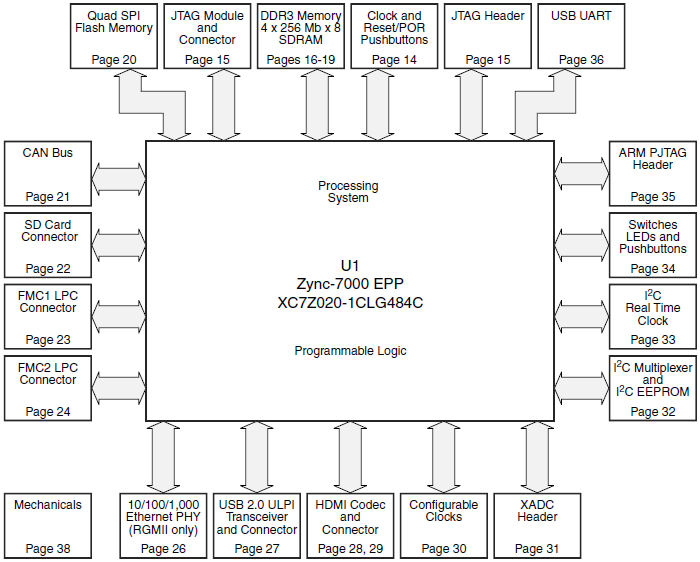
\includegraphics{design/block-diagram}
    }
\end{frame}

%%%%%%%%%%%%%%%%%%%%%%%%%%%%%%%%%%%%%%%%%%%%%%%%%%%%%%%%%%%%%%%%%%%%%%%%%%%%%%%%
% Results
%%%%%%%%%%%%%%%%%%%%%%%%%%%%%%%%%%%%%%%%%%%%%%%%%%%%%%%%%%%%%%%%%%%%%%%%%%%%%%%%
\subsection{Results}
\begin{frame}[label=performance-considerations]{Performance Considerations}
    \begin{itemize}
        \item Cannot transfer data faster than $O(n)$
        \item For each vector that is pruned from the block, we save (on
            average) $\frac{block\_size}{2}$ distance computations
    \end{itemize}
\end{frame}

\begin{frame}[label=performance-estimates]{Performance Estimates}
    The execution time for the proposed design is estimated to be the sum of:
    \begin{enumerate}[<+->]
        \item Execution time of software implementation, excluding the
            distance\_squared function
        \item Time required for DMA transfer of ``outer'' vector.
        \item Time required for DMA transfer of ``inner'' vector, plus the time
            required for the hardware to complete the computation and return the
            result
        \item Overheads associated with thread management
    \end{enumerate}
\end{frame}

%%%%%%%%%%%%%%%%%%%%%%%%%%%%%%%%%%%%%%%%%%%%%%%%%%%%%%%%%%%%%%%%%%%%%%%%%%%%%%%%
% Discussion
%%%%%%%%%%%%%%%%%%%%%%%%%%%%%%%%%%%%%%%%%%%%%%%%%%%%%%%%%%%%%%%%%%%%%%%%%%%%%%%%
\subsection{Discussion}
\begin{frame}[label=discussion]{Discussion}
    \begin{itemize}
        \item Hardware design takes X cycles

        \item On this hardware, we expect a speed-up of X\%

        \item Maximum expected improvement (using Amdahl's Law) is X\%
        \note[item]{Amdahl's Law is used to find the maximum expected
            improvement to an overall system when only part of the system is
            improved. It is often used in parallel computing to predict the
            theoretical maximum speed-up using multiple processors.}

        \item Scaling
    \end{itemize}
\end{frame}